\chapter[Cadeia de Suprimentos ]{Cadeia de Suprimentos}
\label{chap:cadeia}
	
	\section[Definição]{Definição}
	\label{sec:cadeia_definicao}

		A cadeia de suprimentos segundo \cite{martin} “é a rede de organizações envolvidas, por meio de vínculos a montante e a jusante, nos diferentes processos e atividades que produzem valor na forma de produtos e serviços destinados ao consumidor final”. Em outras palavras a cadeia de suprimentos é uma grande teia de aranha que interligada empresas por relações de oferta e demanda, no qual pressupõe uma cadeia de relacionamentos entre fornecedores e clientes, como pode ser ilustrado na imagem a seguir:

		\begin{figure}[h]
			\centering
			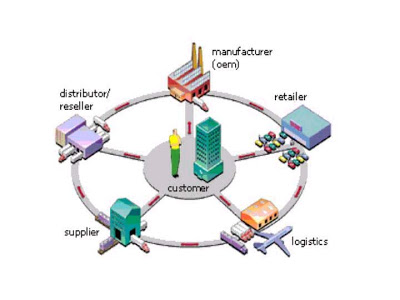
\includegraphics[scale=0.8]{cadeia1}
			\caption[Rede de Operações Produtivas]{Rede de Operações Produtivas.}
			\label{fig:cadeia1}
		\end{figure}

		Em um nível um pouco mais estratégico, a atividade de projeto em administração de produção deve incluir toda a rede da qual uma operação faz parte. Isso porque existem razões pelas quais facilitam todas as perspectivas do negócio. São elas:

		\begin{itemize}
			\item{Ajuda a empresa a compreender como pode competir mais efetivamente;}
			\item{Ajuda a identificar ligações entre nós especialmente significativas na rede;}
			\item{Ajuda a empresa a focalizar uma perspectiva de longo prazo na rede.}
		\end{itemize}

		São essas as razões que auxiliam nas decisões tomadas para configuração de uma rede. Segundo \cite{filho} a decisão de uma cadeia de suprimentos deve ser feita a partir de uma empresa, denominada “empresa focal” ou “empresa foco”. Os membros da cadeia de suprimentos compreendem, nessa visão, todas as organizações com as quais a empresa focal interage direta ou indiretamente através de seus fornecedores ou clientes, desde o ponto de origem até o ponto de consumo. Desse modo, há três dimensões estruturais de uma cadeia de suprimentos, conforme mostra a tabela a seguir.

		\label{subsubsec:cadeia_table}
		\begin{table}[h]
			\centering
			\begin{tabular}{|p{6cm}|p{8cm}|}
				\hline
				\textbf{Dimensões} & \textbf{Definições}  \\ \hline
				Estrutura horizontal & Número de níveis da cadeia de suprimentos. \\ \hline
				Estrutura vertical & Número de empresas em cada nível. \\ \hline
				Posição horizontal da empresa foco dentro da cadeia de suprimentos & A empresa focal pode estar próxima das fontes iniciais de suprimentos, próxima dos clientes finais, ou em alguma posição entre os pontos finais da cadeia. \\ \hline
			\end{tabular}
			\caption[Estrutura da Cadeia de Suprimentos]{Estrutura da Cadeia de Suprimentos. \cite{chopra}}
			\label{tab:cadeia_.table}
		\end{table}

		A cadeia de suprimentos sempre representou um fundamental papel para as empresas, além de ser bastante centrada nas atividades tradicionais como: distribuição física, logística, armazenagem e estoques. De forma simplista, a imagem a seguir ilustra os fluxos de produtos e informações ao longo da rede.

		\begin{figure}[h]
			\centering
			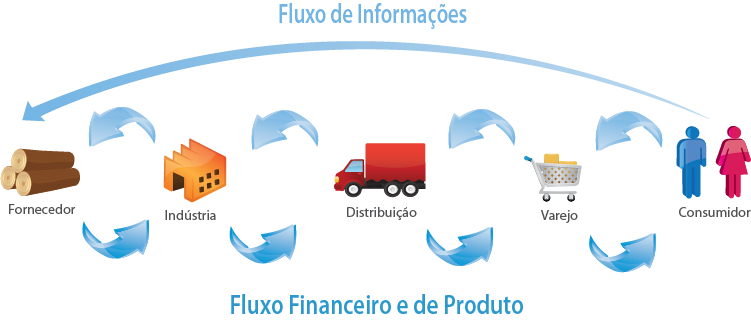
\includegraphics[scale=0.6]{cadeia2}
			\caption[Fluxo de informações e de produtos]{Fluxo de Informações e de Produtos.}
			\label{fig:cadeia2}
		\end{figure}

	\section[Aplicações]{Aplicações - 
\includegraphics{bobs2}}
	\label{sec:cadeia_aplicacoes}

		Agora, atentando-se para a distribuição e logística, de acordo com \cite{junior} a rede \textbf{Bob’s} contém em sua totalidade mais de 620 unidades espalhadas por todos os 26 estados brasileiros e estes importantes números a tornam na rede de \emph{fast food} com a maior cobertura geográfica no país. A rede de restaurantes \textbf{Bob’s} foi de fundamental importância na criação de pontos de venda móvel, sendo uma das pioneiras no mercado brasileiro. Implantaram inicialmente as mini lojas que eram feitas de aço com apenas 23 metros quadrados, que foram projetadas especificamente para ser colocada em qualquer lugar bastante movimentado como: praças, ruas e estacionamentos, e os chamados quiosques, atualmente com mais de 230 unidades de 15 metros quadrados, apropriadas para os corredores dos shoppings.

		Ainda de acordo com \cite{lamonica} em seu livro, o sabor de uma marca: \textbf{Bob’s} 60 anos, um grande feito do \textbf{Bob’s} foi unir suas lanchonetes a postos de conveniência que hoje já totalizam 52 lojas, utilizando o conceito \emph{“store in store”}\footnote{Tecnicamente, \emph{store in store} é quando se cria um espaço comercial específico de terceiros dentro do nosso chão de loja, em sinergia com o nosso negócio, visando ampliar, focalizar ou aprofundar a oferta de bens e serviços para o nosso cliente. (D.D Consultoria de Negócios, 2012)}, a rede descobriu um potencial de lucro ainda inexplorado pelas outras redes e possui lojas nos principais aeroportos do Brasil que atendem 24 horas. O \textbf{Bob’s} possui, além de tudo, um moderno e sofisticado sistema de entrega de pedidos que, para ser realizado com eficiência, necessita que o cliente se cadastre no site para a verificação de pedido e escolha da forma de pagamento, e também verificar se a sua residência encontra-se em uma das localidades atendidas dentro dos 12 estados que possuem o \textbf{Bob’s \emph{Delivery}}. O \textbf{Bob’s} tem uma política justa de tempo máximo de 40 minutos para a entrega do pedido.

		Para abastecer os suprimentos de toda essa rede com lojas localizadas nos mais diversos lugares e continuar progredindo, a empresa, recentemente, resolveu melhorar seu sistema de distribuição. Com essa melhoria, todas as regiões vão ter um sistema de abastecimento com qualidade equilibrada e de alto padrão.  A rede assinou um contrato com a TGB, uma empresa com especialidade no transporte de alimentos do tipo \emph{fast food}. Com esse novo sistema os custos de distribuição serão reduzidos em aproximadamente 20\%.

		A rede de franquias tem, atualmente, a sua gestão da cadeia de suprimentos terceirizada. No ano de 2011 a empresa que passou a ter essa função foi a \textbf{Martin Brower}, empresa com o relacionamento do tipo negócio a negócio, reconhecida no mercado por trabalhar com a rede \emph{Mc Donald’s} nos Estados Unidos por mais de 50 anos. Ela é responsável por todo processo entre os produtores de matérias-primas e as lojas, fazendo a compra dos produtos, transporte, gestão de estoque, armazenamento e entrega.

		\begin{quotation}
			“Nosso foco é oferecer sempre o melhor produto ao cliente. Optamos por uma empresa com o \emph{know-how} da Martin-Brower por entendermos que o processo de distribuição e armazenamento é um fator muito importante na manutenção da qualidade dos nossos produtos.” \cite{detsi}
		\end{quotation}
		
		A empresa faz uso do sistema \emph{WOP – Web Order Planing}, uma ferramenta que equaliza os estoques e facilita a emissão de pedidos da loja para a \textbf{Martin Brower}. Esse sistema analisa o estoque do restaurante, histórico de vendas e faz uma previsão de vendas futuras, tudo para garantir o melhor aproveitamento dos estoques da loja. A ilustração a seguir apresenta fundamentalmente o funcionamento deste sistema. 

		\begin{figure}[h]
			\centering
			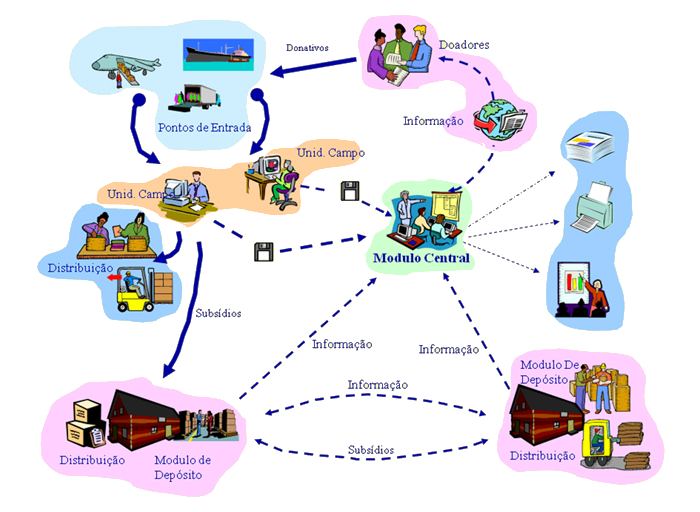
\includegraphics[scale=0.6]{cadeia3}
			\caption[Esquema de Comunicação WOP]{Esquema de Comunicação WOP.}
			\label{fig:cadeia3}
		\end{figure}

		Por ter uma demanda com baixo erro de previsão e produtos que possuem pequeno prazo de validade, a empresa usa uma estratégia de cadeias de suprimento eficientes, mantendo estoques operando no mínimo e priorizando baixo custo, qualidade constante e entrega pontual.	

		O diagrama a seguir ilustra uma simplificação da cadeia de suprimentos do \textbf{Bob’s} e a participação da \textbf{Martin Brower} no processo.

		\newpage
		\begin{figure}[h]
			\centering
			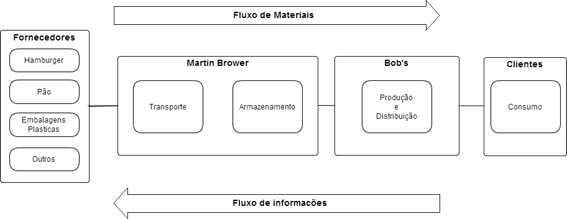
\includegraphics[scale=0.5]{cadeia4}
			\caption[Diagrama da cadeia de suprimentos Bob's - Martin Brower]{Diagrama da cadeia de suprimentos \textbf{Bob’s} - \textbf{Martin Brower}.}
			\label{fig:cadeia4}
		\end{figure}

		Com a gestão da cadeia de suprimentos terceirizada, a rede \textbf{Bob’s} pode focar na inovação dos serviços e produtos, melhor atendimento e satisfação dos seus clientes.